\documentclass[12pt]{article}

% This is all the packages and settings and so on.
% It is using custom fonts that needs to be installed on the computer. If they are not present, they have to be added manually.
\usepackage[
	citestyle=ieee, 
    bibstyle=ieee,
    style=numeric-comp,
    sorting=nty, 
%     sortcites=true
    ]{biblatex}
    
% Makes the last name first in the bibliography.
\DeclareNameAlias{author}{last-first}
    
% Specify the margins
\usepackage[a4paper, margin=3cm]{geometry}

\usepackage{eso-pic}								% Packages for layout and graphics 
\usepackage{graphicx}
\usepackage{tikz}
\usepackage{setspace}
\usepackage{tocloft}		 						% Fixing a bug with page style changes for toc
\tocloftpagestyle{fancy}
\usepackage{etoc} 									%Separate tocs for appendix and the rest    
\usepackage{chngcntr}							  	% Count figures within chapters
\counterwithin{figure}{section} 
\counterwithin{table}{section}
\usepackage{booktabs}							  	% Table formatting
\usepackage{fancyhdr}								% Setting the style for header and footer.
\usepackage[hidelinks]{hyperref}					% Clickable links
\usepackage{nameref}								% References with names
\usepackage[parfill]{parskip}						% New line instead of indent for sections
\usepackage{subfig}						 			% Package for putting figures side by side
\usepackage{tcolorbox}								% Create boxes around content
\tcbset{colback=white,arc=0mm}

% Specifying fonts
\usepackage{fontspec}
\setmainfont{Georgia} 
\setsansfont{Arial}
\newfontfamily\footerfont{Georgia}

\usepackage{sectsty}
\sectionfont{\sffamily\fontsize{14}{15}}
\subsectionfont{\sffamily\fontsize{13}{15}}
\subsubsectionfont{\sffamily\fontsize{12}{15}}

% Remove the title and make sure that the text is adjusted
\usepackage{abstract}
\setlength{\absleftindent}{0mm}
\renewcommand{\abstractname}{\vspace{-\baselineskip}}
\renewcommand{\abstractnamefont}{\sffamily\fontsize{14}{15}}
\renewcommand{\abstracttextfont}{\normalfont\fontsize{12}{13}}

% Renaming and setting style of table of contents
\usepackage{tocloft}
\renewcommand*\contentsname{Contents}
\renewcommand*\cfttoctitlefont{\fontsize{16}{0}\bf\sffamily}
\renewcommand\cftsecfont{\fontsize{12}{0}\bf\sffamily}
\renewcommand\cftsecpagefont{\fontsize{12}{0}\bf\sffamily}


% Styling the header and footer
\pagestyle{fancy}
\fancyhf{}
\renewcommand{\headrulewidth}{0pt}
\fancyfoot[R]{\footerfont\thepage}

% Making the command for placing text in random locations
\newcommand\PlaceText[3]{%
\begin{tikzpicture}[remember picture,overlay]
\node[outer sep=0pt,inner sep=0pt,anchor=south west] 
  at ([xshift=#1,yshift=-#2]current page.north west) {#3};
\end{tikzpicture}%
}

% Disable hyphenation
\pretolerance=10000
\tolerance=2000 
\emergencystretch=500pt

% Custom toc for cleaner main document
\newcommand{\customtoc}{
        \etocdepthtag.toc{mtchapter}
        \etocsettagdepth{mtchapter}{subsection}
        \etocsettagdepth{mtappendix}{none}
        \newpage
        \thispagestyle{fancy}
        \tableofcontents
        % Fixing a bug where the page number would randomly fail to be right justified.
        \thispagestyle{fancy} 
        \newpage
}

% Defining files for bibliography
%\addbibresource{ref.bib}
\addbibresource{references.bib}
% Add a second bibliography file for the second author to allow
% both to update it through the mendeley integration.
% \addbibresource{ref-author-2.bib}

% Defining document information
\title{Template}
\newcommand{\subtitle}{KTH Bachelor Thesis Report}
\author{<Author Name and Author Name>}

\begin{document}
\setstretch{1.4}

% The front page of the document
\makeatletter
\begin{titlepage}

\vspace*{-4.6\baselineskip}
\hspace*{-0.15\textwidth}
\includegraphics[width=0.2\paperwidth]{img/kth-logo}%
\par\vspace*{2.5\baselineskip}

\PlaceText{65mm}{12mm}{\fontsize{12}{0}\sffamily DEGREE PROJECT IN TECHNOLOGY,}
\PlaceText{65mm}{17mm}{\fontsize{12}{0}\sffamily FIRST CYCLE, 15 CREDITS}
\PlaceText{65mm}{22mm}{\fontsize{12}{0}\sffamily\itshape STOCKHOLM, SWEDEN \the\year}

~\\

\hspace*{-3cm}\begin{minipage}[b]{63.5mm}
~\\
\end{minipage}
\begin{minipage}{0.65\textwidth}
\begin{flushleft}
{\fontsize{28}{24}\bf\sffamily\@title\\}
\vspace{0.5cm}
{\fontsize{19}{17}\bf\sffamily \subtitle\\}
\vspace{0.5cm} 
{\fontsize{16}{0}\sffamily \@author}\\
\end{flushleft}

\end{minipage}


\AddToShipoutPictureBG*{%]
    \AtPageLowerLeft{%
        
\includegraphics[width=1.0\paperwidth]{img/kth-footer}%
    }%
}

\PlaceText{65mm}{280mm}{\color{white}\fontsize{12}{0}\sffamily KTH ROYAL INSTITUTE OF TECHNOLOGY }
\PlaceText{65mm}{285mm}{\color{white}\fontsize{8}{0}\sffamily ELECTRICAL ENGINEERING AND COMPUTER SCIENCE }
\end{titlepage}
\makeatother


\newpage
\pagenumbering{roman}

\newpage

%%%%%%%%%%%%%%%%%%%%%%%%%%%%%%%%%%%%
%%														 The English abstract						            		%%
%%%%%%%%%%%%%%%%%%%%%%%%%%%%%%%%%%%%
\section*{Abstract}
%%%%%%%%%%%%%%%%%%%%%%%%%%%%%%%%%%%%

This is a template for writing bachelor thesis reports for the ICT school at KTH. I do not own any of the images provided in the template and this can only be used to submit thesis work for KTH.

The report needs to be compiled using XeLaTeX as different fonts are needed for the project to look like the original report. You might have to change this manually in overleaf.

This template was created by Hannes Rabo <hannes.rabo@gmail.com or hrabo@kth.se> from the template provided by KTH. You can send me an email if you need help in making it work for you.


\vspace{2cm}
Write an abstract. Introduce the subject area for the project and describe the problems that are solved and described in the thesis. Present how the problems have been solved, methods used and present results for the project. Use probably one sentence for each chapter in the final report.

The presentation of the results should be the main part of the abstract. Use about ½ A4-page.
English abstract




\subsection*{Keywords}
Template, Thesis, Keywords ...






\newpage
%%%%%%%%%%%%%%%%%%%%%%%%%%%%%%%%%%%%
%%														 The Swedish abstract								         %%
%%%%%%%%%%%%%%%%%%%%%%%%%%%%%%%%%%%%
\section*{Abstract}
%%%%%%%%%%%%%%%%%%%%%%%%%%%%%%%%%%%%
Svenskt abstract
Svensk version av abstract – samma titel på svenska som på engelska.

Skriv samma abstract på svenska. Introducera ämnet för projektet och beskriv problemen som löses i materialet. Presentera 

\subsection*{Nyckelord}
Kandidat examensarbete, ...


\newpage
\section*{Acknowledgements}
Write a short acknowledgements. Don't forget to give some credit to the examiner and supervisor.






\newpage
\thispagestyle{empty}
This page is very optional
~\\
\vfill
{ \setstretch{1.1}
	\subsection*{Authors}
	Author Name <email@domain.com> and Author Name\\
	Information and Communication Technology\\
	KTH Royal Institute of Technology
	
	\subsection*{Place for Project}
	Stockholm, Sweden\\
	Some place
	
	\subsection*{Examiner}
	The Professor
	Place \\
	KTH Royal Institute of Technology
	
	\subsection*{Supervisor }
	The Supervisor\\
	Place\\
	KTH Royal Institute of Technology
	~
	
}




% The table of content
\customtoc

The content only includes the first level of sub-headings as the third level was less relevant in the scope of the entire report. This can be changed in the setup.tex file.

\pagenumbering{arabic}

\section{Introduction}

Provide a general introduction to the area for the degree project. Use references!

Link things together with references. This is a reference to a section: \ref{sec:background}.

\subsection{Background}
\label{sec:background}
Present the background for the area. Give the context by explaining the parts that are needed to understand the degree project and thesis. (Still, keep in mind that this is an introductory part, which does not require too detailed description).

Use references\footnote{You can also add footnotes if you want to clarify the content on the same page.}

Detailed description of the area should be moved to Chapter 2, where detailed information about background is given together with related work. 

This background presents background to writing a report in latex.


Example citation \cite{Jones2017} or for two authors: \cite{Jones2017, Liu2017}

Look at sample table \ref{tab:sample-table-label} for a table sample.

\begin{table}[!ht]
\centering
\caption{Sample table. Make sure the column with adds up to 0.94 for a nice look.}
~\\
\label{tab:sample-table-label}
\begin{tabular}{p{0.3\textwidth} p{0.64\textwidth}}
\toprule
\textbf{SAMPLE}		  & \textbf{TABLE}                                                                                                                                                  \\ \toprule
One                   & Stuff 1 \\
\midrule
Two                   & Stuff 2 \\
\midrule
Three                 & Stuff 3\\
\bottomrule
\end{tabular}
\end{table}



Boxes can be used to organize content

\begin{tcolorbox}[title={Development environment for prototype}]
	\tt{
		\textbf{Operating systems }\\
		computer: Linux - kernel 4.18.5-arch1-1-ARCH\\
		android phone: 8.1.0\\
		~\\
		\textbf{Build tools}\\
		exp (build tool): version 55.0.4\\
		~\\
		...
	}
\end{tcolorbox}


Multiple images can be placed side by side like this:
\begin{figure}[ht]
	\centering 
	\subfloat[First subfigure]{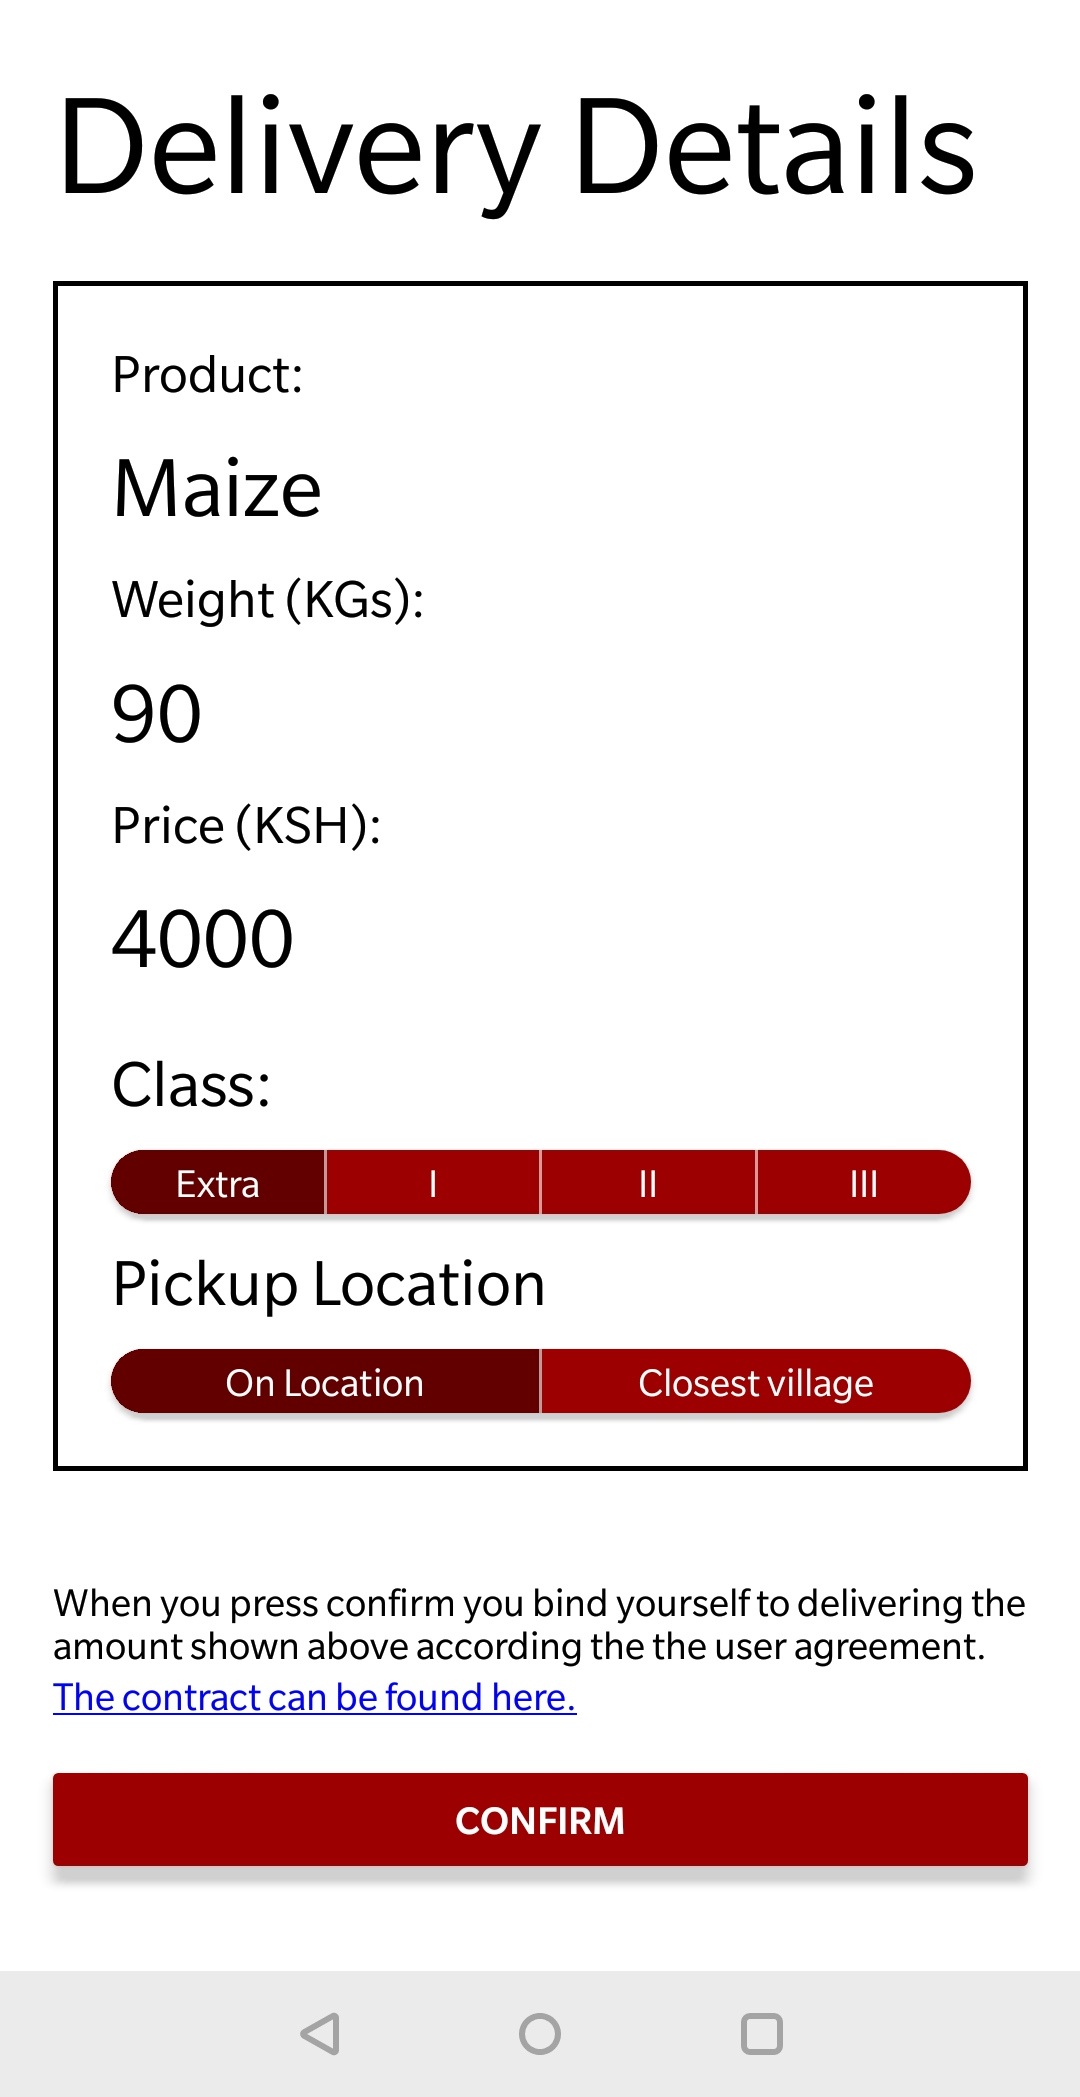
\includegraphics[width=0.3\textwidth]{img/sample-image}
		\label{fig:sample-image:1}}
	\hfill
	\subfloat[Second subfigure]{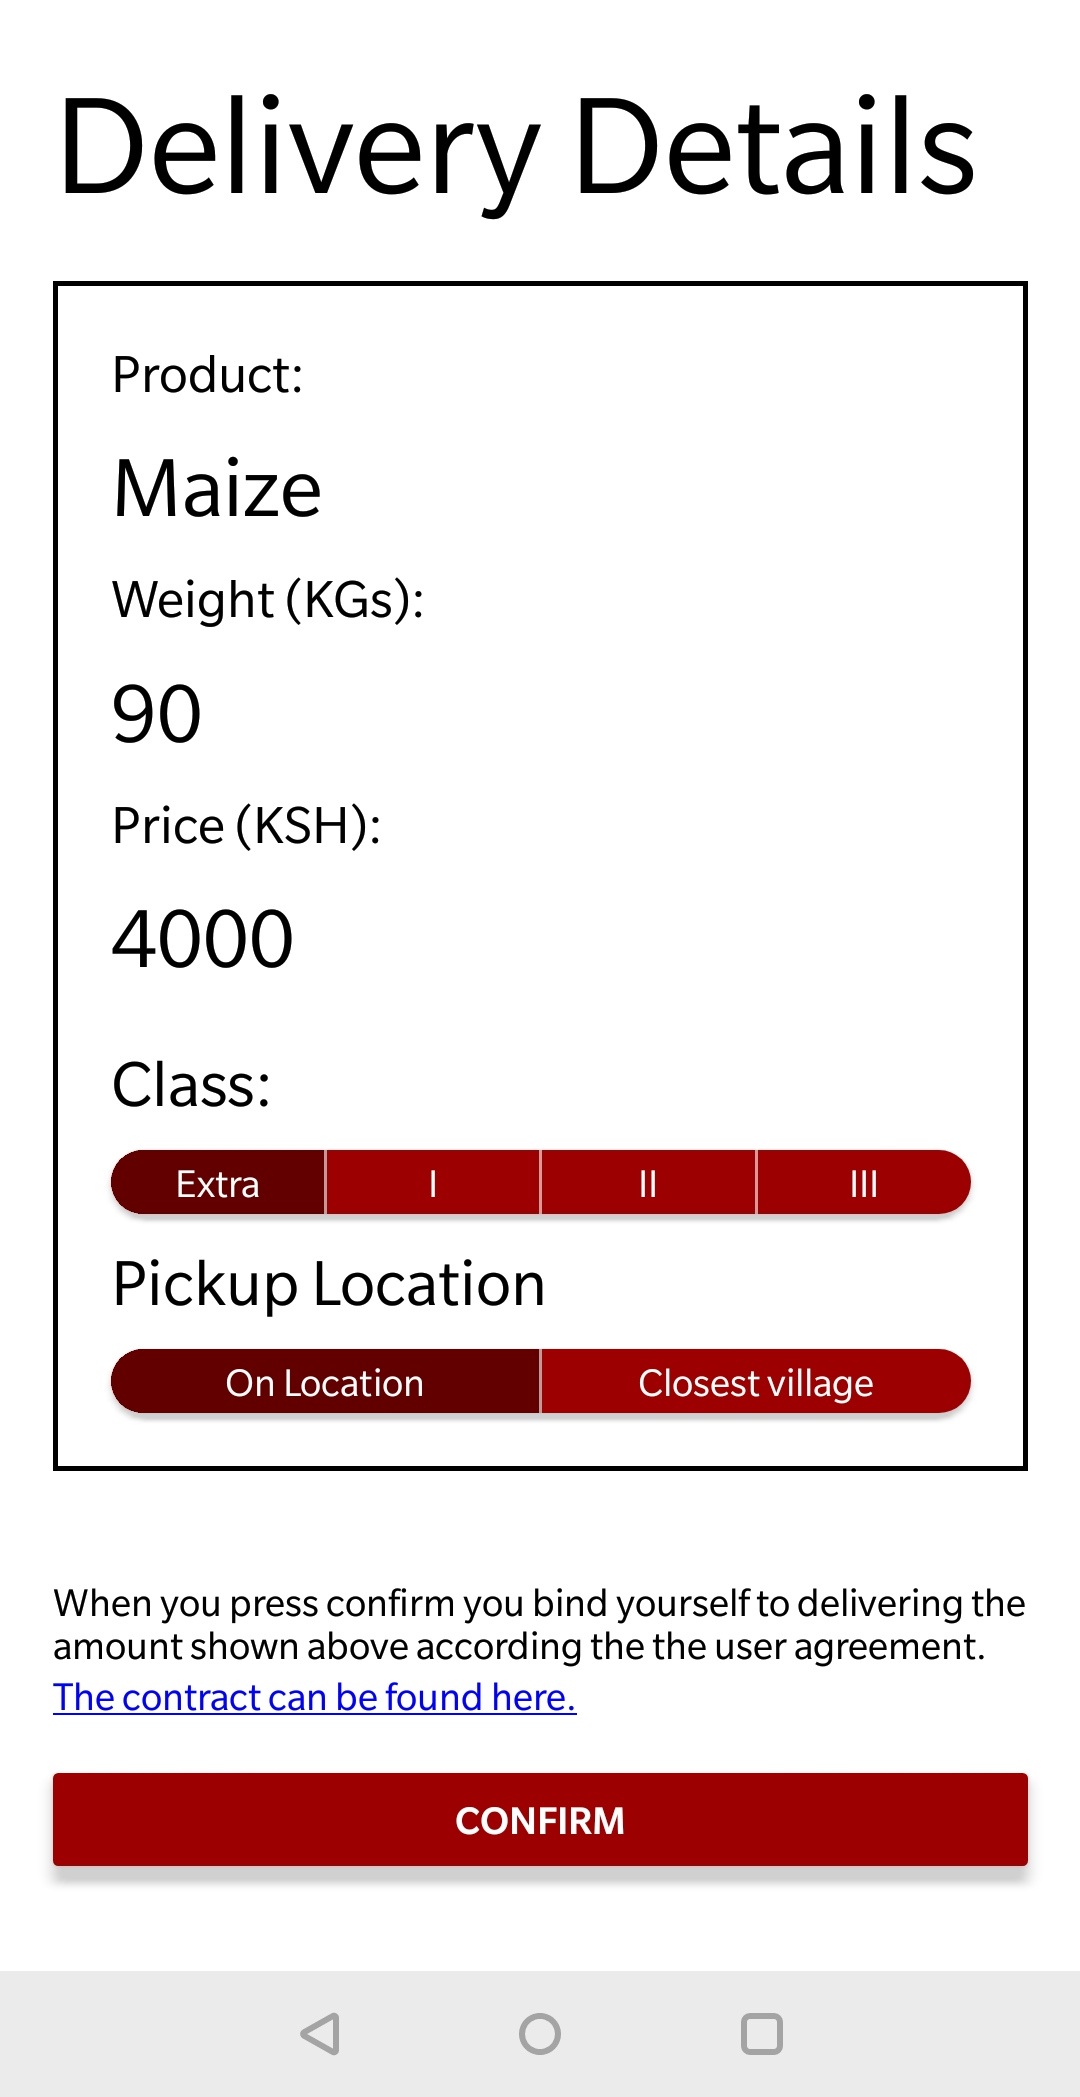
\includegraphics[width=0.3\textwidth]{img/sample-image}
		\label{fig:sample-image:2}}
	\hfill
	\subfloat[Third subfigure]{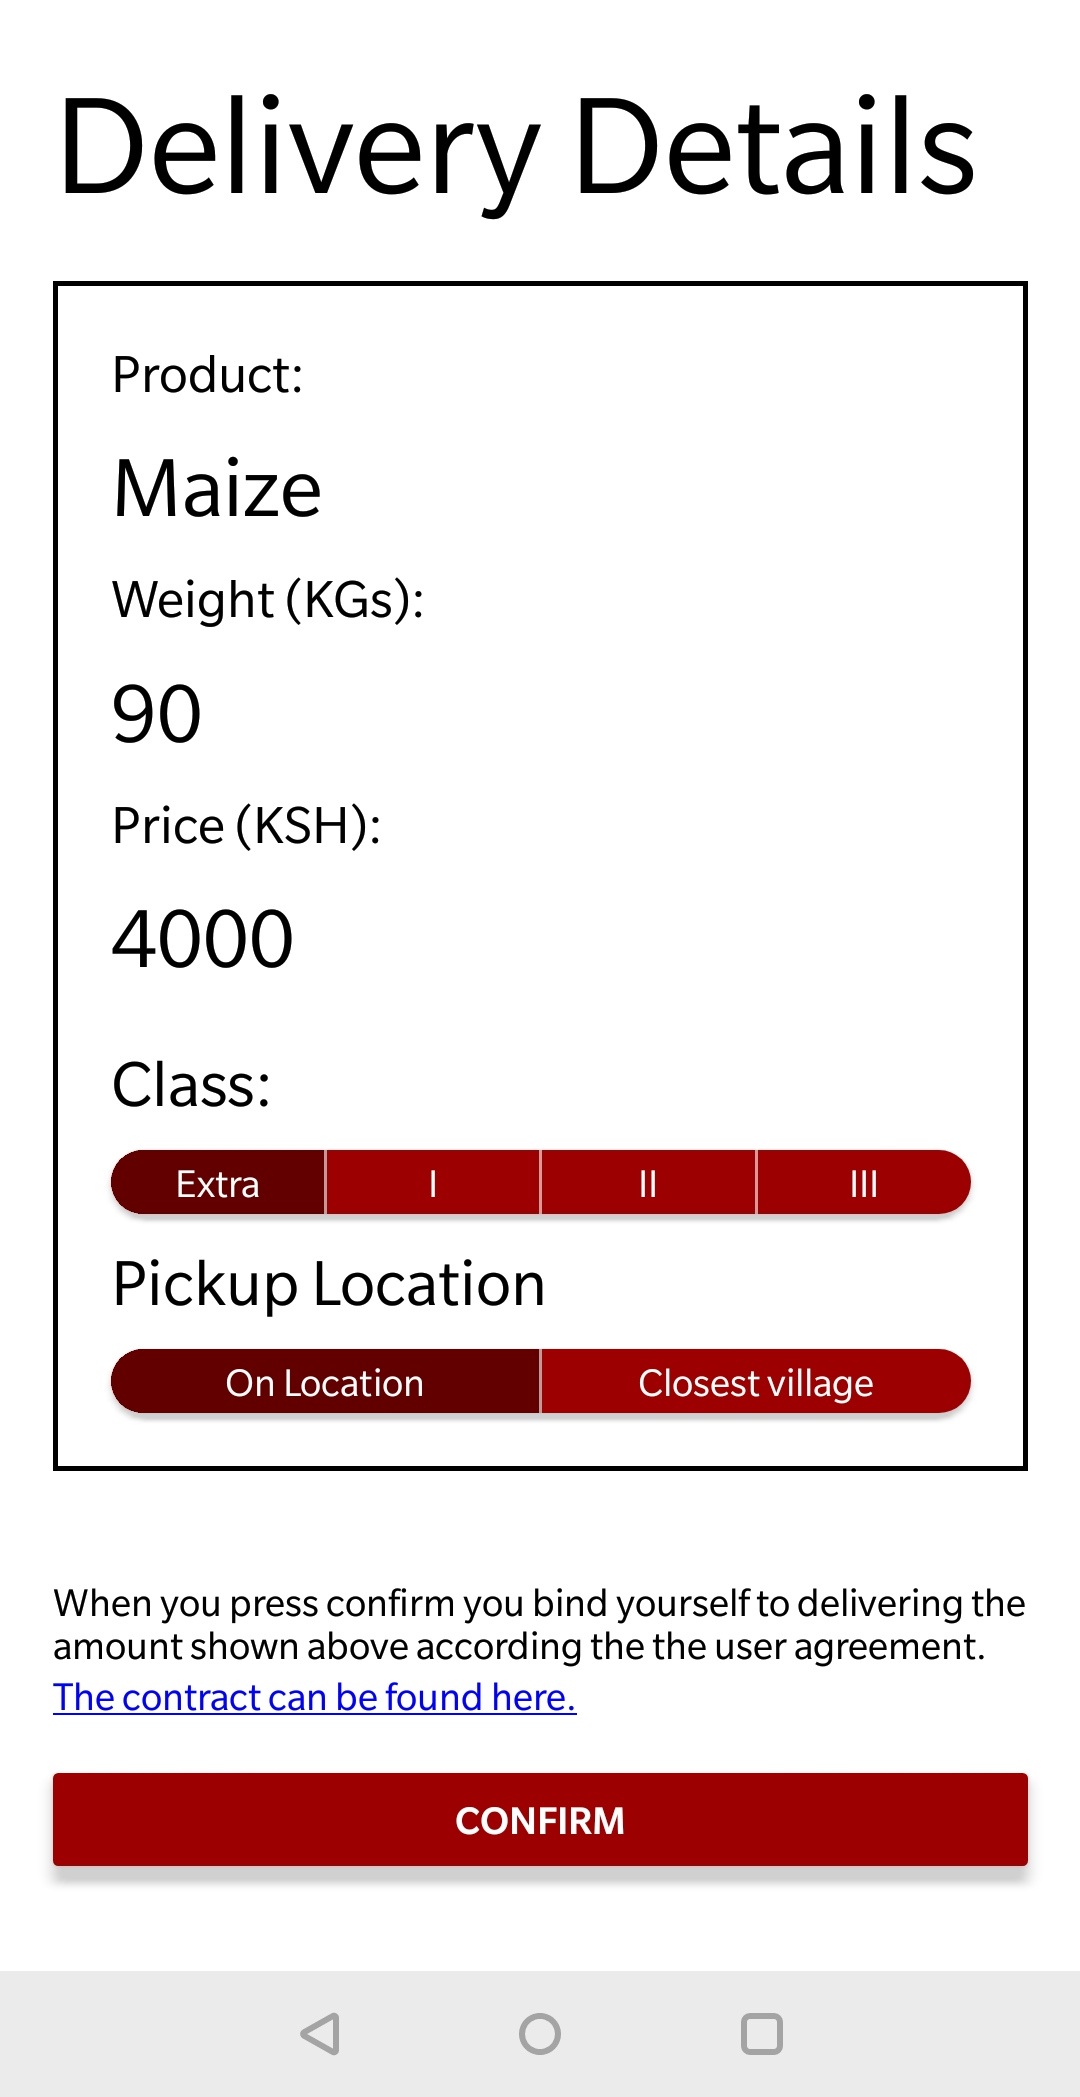
\includegraphics[width=0.3\textwidth]{img/sample-image}
		\label{fig:sample-image:3}}
	\caption{\textit{General figure caption. The width might not add up to 1. Try make sure it adds up to 0.9 instead.}}
\end{figure}

\subsection{Problem}
Present the problems found in the area. Preferable use and end this section with a question as a problem statement.

Use references
Preferable, state the problem, to be solved, as a question. Do not use a question that can be answered with yes and/or no. 

\subsection{Purpose}
The purpose of the degree project/thesis is the purpose of the written material, i.e., the thesis. The thesis presents the work / discusses / illustrates and so on.

It is not “The project is about” even though this can be included in the purpose. If so, state the purpose of the project after purpose of the thesis).

\subsection{Goal}
The goal means the goal of the degree project. Present following: the goal(s), deliverables and results of the project. 

\subsubsection{Benefits, Ethics and Sustainability}
Describe who will benefit from the degree project, the ethical issues (what ethical problems can arise) and the sustainability aspects of the project.

Use references!

\subsection{Methodology}
Introduce, theoretically, the methodologies and methods that can be used in a project and, then, select and introduce the methodologies and methods that are used in the degree project. Must be described on the level that is enough to understand the contents of the thesis. 

Use references!

Preferably, the philosophical assumptions, research methods, and research approaches are presented here. Write quantitative / qualitative, deductive / inductive / abductive. Start with theory about methods, choose the methods that are used in the thesis and apply. 


Detailed description of these methodologies and methods should be presented in Chapter 3. In chapter 3, the focus could be research strategies, data collection, data analysis, and quality assurance.


\subsection{Stakeholders}
Present the stakeholders for the degree project.

\subsection{Delimitations}
Explain the delimitations. These are all the things that could affect the study if they were examined and included in the degree project. 
Use references!

\subsection{Outline}
In text, describe what is presented in Chapters 2 and forward. Exclude the first chapter and references as well as appendix. 

\section{<Theoretical Background>}
In this chapter, a detailed description about background of the degree project is presented together with related work. Discuss what is found useful and what is less useful. Use valid arguments. 

Explain what and how prior work / prior research will be applied on or used in the degree project /work (described in this thesis). Explain why and what is not used in the degree project and give valid reasons for rejecting the work/research.

Use references!

\subsection{Use headings to break the text}
Do not use subtitles after each other without text in between the sections.

\subsection{Related Work}
You should probably keep a heading about the related work here even though the entire chapter basically only contains related work.

\section{<Engineering-related content, Methodologies and Methods>}
Describe the engineering-related contents (preferably with models) and the research methodology and methods that are used in the degree project. 

Most likely it generally describes the method used in each step to make sure that you can answer the research question.

\subsection{Engineering-related and scientific content:}
Applying engineering related and scientific skills; modelling, analysing, developing, and evaluating engineering-related and scientific content; correct choice of methods based on problem formulation; consciousness of aspects relating to society and ethics (if applicable).

As mentioned earlier, give a theoretical description of methodologies and methods and how these are applied in the degree project.

\section{<The Work> }
Describe the degree project. What did you actually do? This is the practical description of how the method was applied.

\section{<Result> }
Describe the results of the degree project.

\section{<Conclusions> }
Describe the conclusions (reflect on the whole introduction given in Chapter 1). 

Discuss the positive effects and the drawbacks. 

Describe the evaluation of the results of the degree project.

Describe valid future work.  

The sections below are optional but could be added here.

\subsection{Discussion}

\subsection{Future Work}

\subsection{Final Words}









% \include{content}

\newpage
\addcontentsline{toc}{section}{References}
\textbf{If you are using mendeley to manage references, you might have to export them manually in the end as the automatic ways removes the "date accessed" field}
\printbibliography


\newpage
\section*{Appendices}
\appendix
\newpage
\etocdepthtag.toc{mtappendix}
\etocsettagdepth{mtchapter}{none}
\etocsettagdepth{mtappendix}{subsection}
\etoctocstyle{1}{Appendix - Contents}
\tableofcontents
\newpage


\section{First Appendix}
This is only slightly related to the rest of the report


\section{Second Appendix}
this is the information


\newpage
% This is the last page of the document
\thispagestyle{empty}
\AddToShipoutPictureBG*{%]
    \AtPageLowerLeft{%
        
\includegraphics[width=1.0\paperwidth]{img/kth-footer}%
    }%
}

\PlaceText{20mm}{282mm}{\color{white}\fontsize{12}{0}\sffamily www.kth.se }


\end{document}
